\documentclass{article}
\usepackage{graphicx}
\begin{document}

\title{
Bryan Petzinger \\
Computer Vision \\
HW3 \\
}
\maketitle

\section{Writeup}
brief description \\
performance \\
works correctly? \\
specific techniques (implementation) \\
suprises/difficulties/observations \\

\section{Figures}

\begin{figure}[h]
\caption{}
\centering
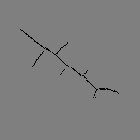
\includegraphics{images/skeleton.jpg}
\end{figure}

\begin{figure}[h]
\caption{}
\centering

\includegraphics{images/rebuilt_image10.jpg}
\end{figure}

\begin{figure}[h]
\caption{}
\centering

\includegraphics{images/rebuilt_image9.jpg}
\end{figure}

\begin{figure}[h]
\caption{}
\centering

\includegraphics{images/rebuilt_image8.jpg}
\end{figure}

\begin{figure}[h]
\caption{}
\centering
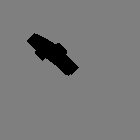
\includegraphics{images/rebuilt_image7.jpg}
\end{figure}

\begin{figure}[h]
\caption{}
\centering

\includegraphics{images/rebuilt_image6.jpg}
\end{figure}

\begin{figure}[h]
\caption{}
\centering

\includegraphics{images/rebuilt_image5.jpg}
\end{figure}

\begin{figure}[h]
\caption{}
\centering
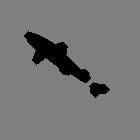
\includegraphics{images/rebuilt_image4.jpg}
\end{figure}

\begin{figure}[h]
\caption{}
\centering
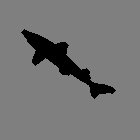
\includegraphics{images/rebuilt_image3.jpg}
\end{figure}

\begin{figure}[h]
\caption{}
\centering
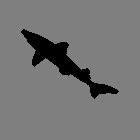
\includegraphics{images/rebuilt_image2.jpg}
\end{figure}

\begin{figure}[h]
\caption{}
\centering
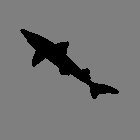
\includegraphics{images/rebuilt_image1.jpg}
\end{figure}

\begin{figure}[h]
\caption{}
\centering
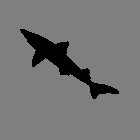
\includegraphics{images/rebuilt_image0.jpg}
\end{figure}








\end{document}
